En la actualidad se ha vuelto un problema cotidiano para los conductores de veh�culos particulares encontrar un estacionamiento con lugares disponibles, principalmente en zonas comerciales, de oficinas o con gran actividad econ�mica. Es com�n que un conductor vaya a un estacionamiento en espec�fico y no tenga espacios disponibles, lo cual, puede hacer que pierda un tiempo considerable en esperar a que se libere alg�n caj�n para poder alojar su veh�culo.

Del mismo modo, para due�os de estacionamientos los ingresos no son suficientes para la adquisici�n de un sistema o la contrataci�n de  un  agente externo que realice dicha administraci�n y/o automatizaci�n; incluso para estacionamientos grandes con mayores ingresos la implementaci�n de un sistema, automatizaci�n u outsourcing disminuye en gran medida sus ingresos. Una cotizaci�n realizada con un de las empresas con mayor impacto en el mercado mexicano para la gesti�n de estacionamientos, Ranver \texttrademark. Revel� que los due�os de estacionamientos al contratar estos servicios tardan entre 1 y 2 a�os para percibir ganancias, pasado este tiempo las ingresos mensuales se reparten 50\% para el due�o y 50\% para Ranver\texttrademark. 

Finalmente, no existe una herramienta, donde, los administradores de estacionamientos puedan gestionar su estacionamiento y al mismo tiempo publiquen su informaci�n en tiempo real(ubicaci�n, horarios, n�mero de cajones, n�mero de cajones disponibles, servicios, establecimientos, tarifas, Etc.) a potenciales clientes. Por otra parte, los conductores de veh�culos es muy probable que no conozcan todos los estacionamientos cerca de ubicaci�n actual cuando necesite un lugar donde alojar su veh�culo, ni mucho menos su ocupabilidad, tarifas, servicios, Etc. Adem�s no hay herramientas que agilicen y ayuden a la gesti�n y comunicaci�n entre administrador y usuario final.   


Todos estos problemas traen consigo otras dificultades. Una investigaci�n realizada por el Instituto de Pol�ticas para el Transporte y el Desarrollo (ITDP), revel� que en �reas d�nde la oferta de estacionamientos no es suficiente para cubrir la demanda y se ofrecen espacios de estacionamiento en v�a p�blica de manera gratuita, se generan efectos negativos que afectan a residentes y visitantes \cite{ITDP}.

\begin{figure}[h]
	\centering
	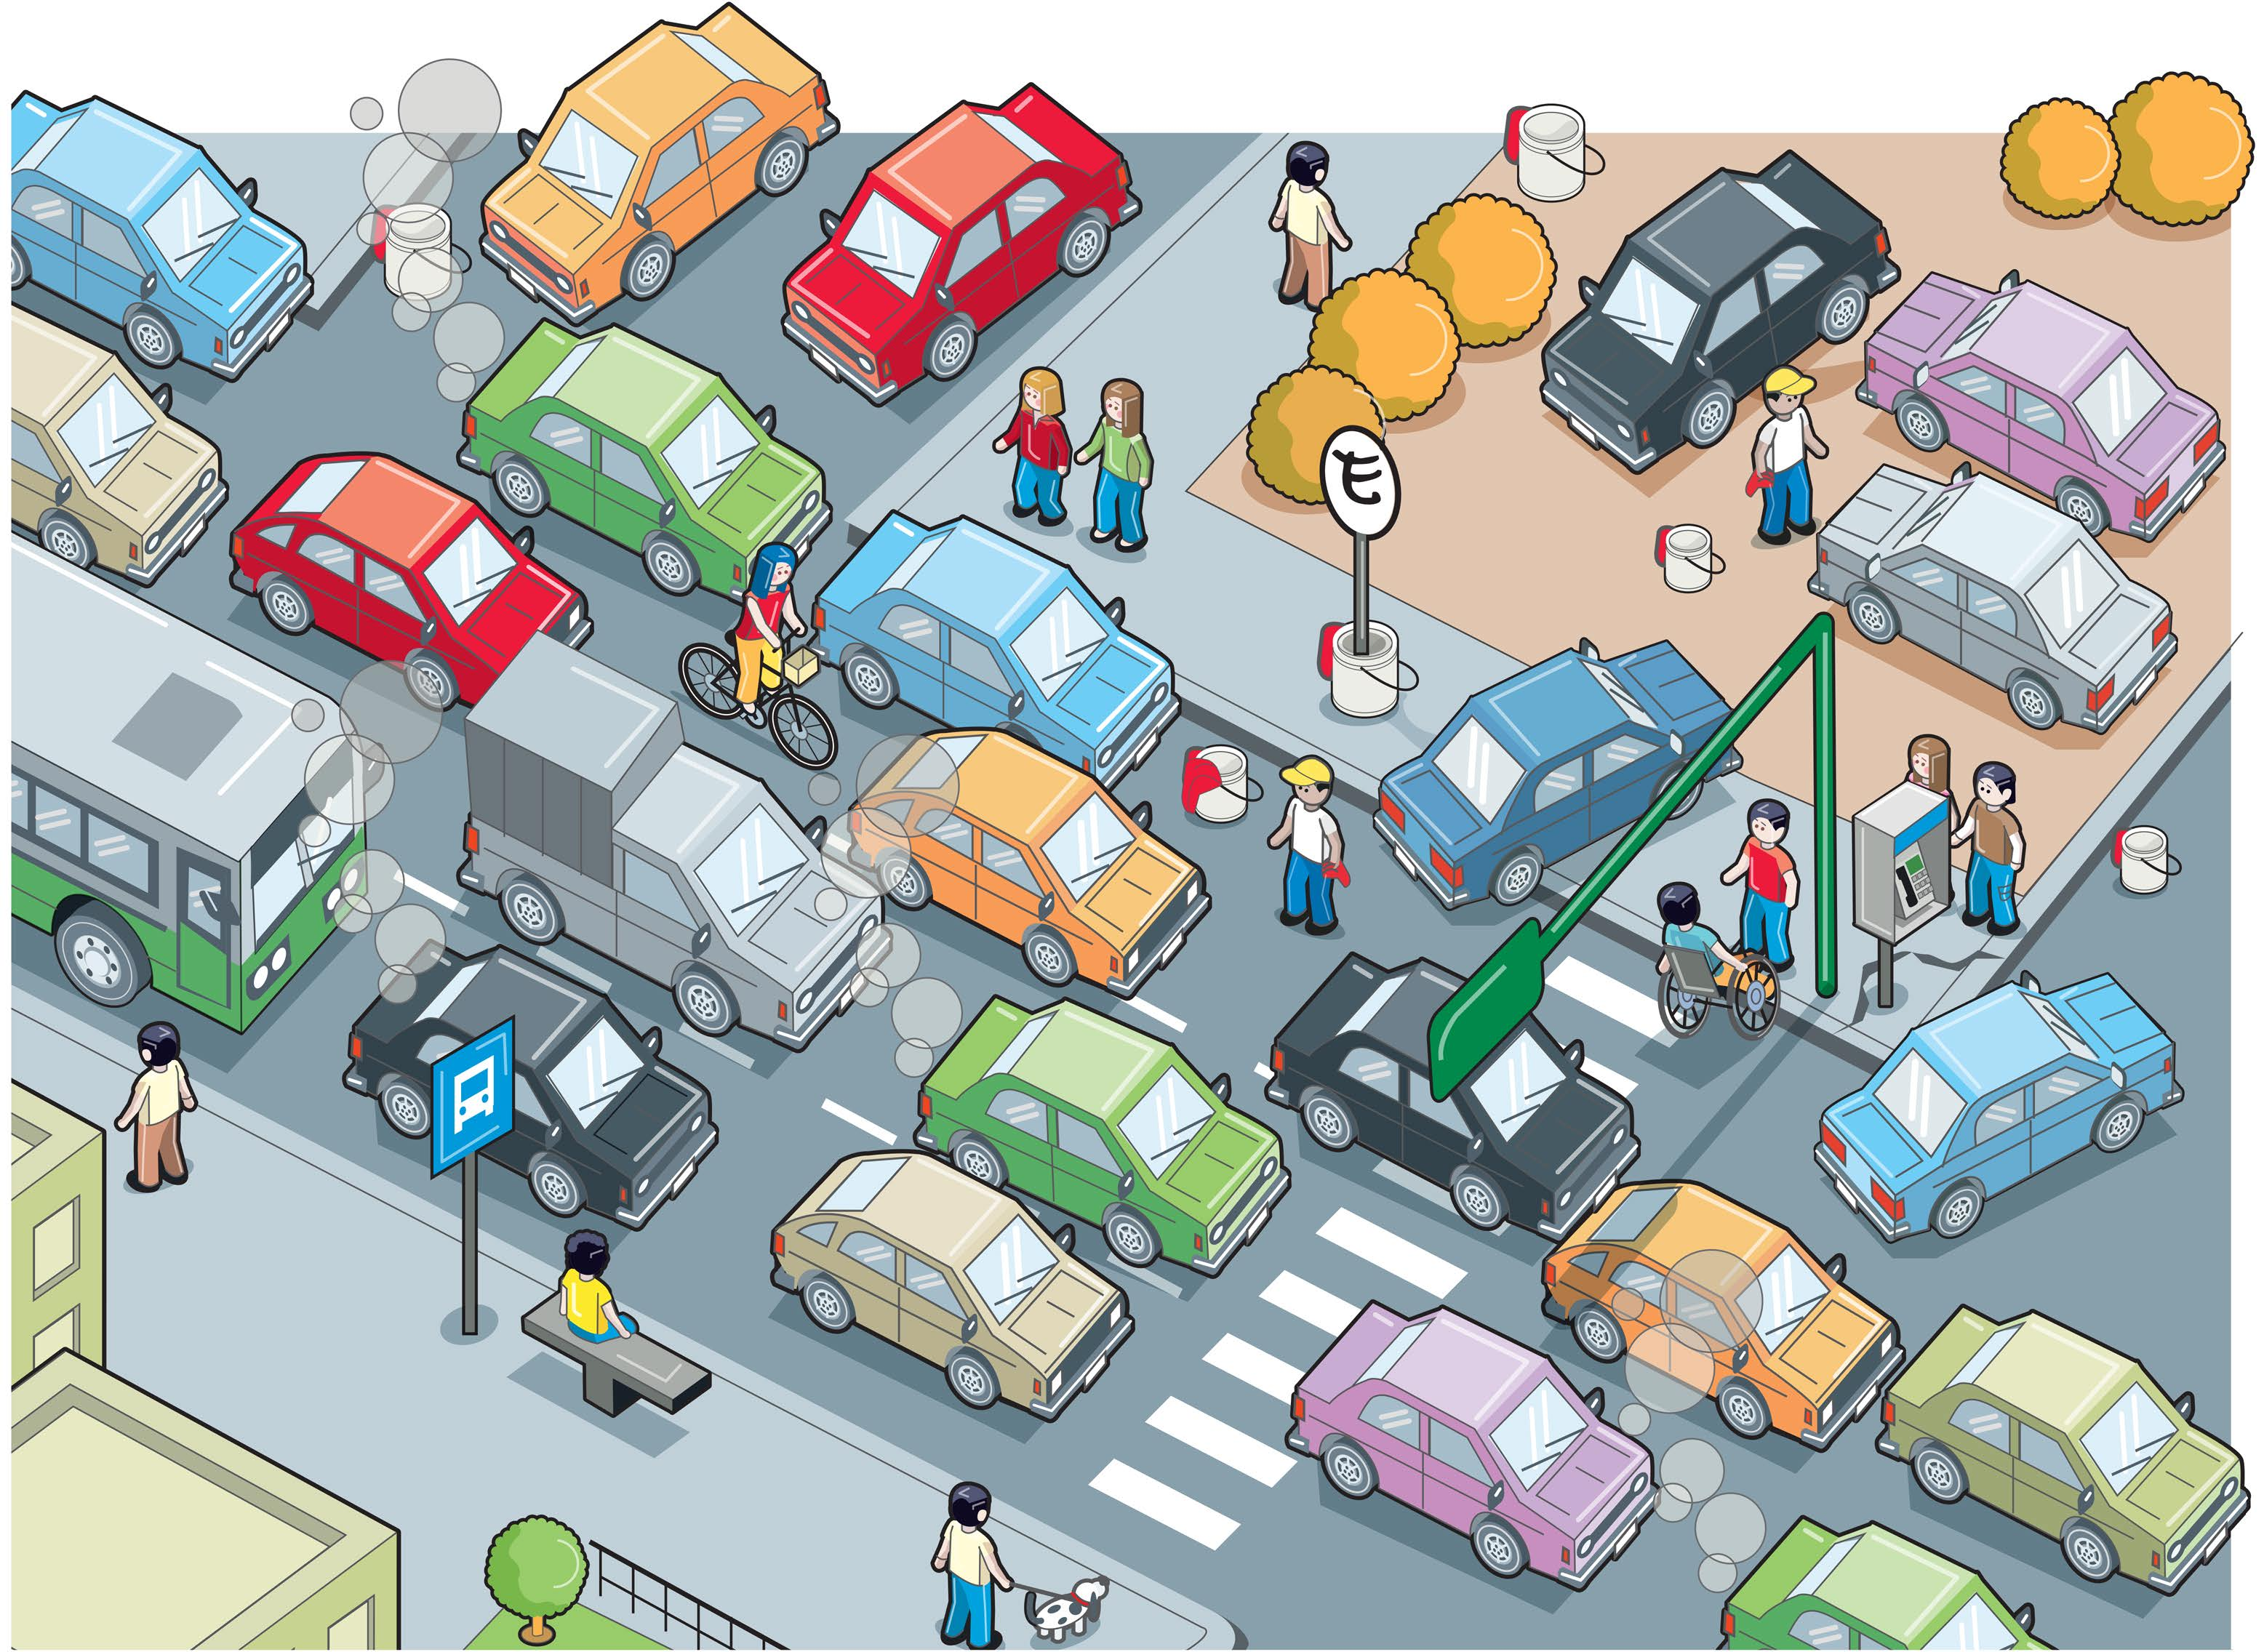
\includegraphics[scale=.15]{./estudioDeMercado/definicionDelProblema/source/trafico.pdf}
	\caption{Problemas cotidianos por falta disponibilidad en estacionamientos}
	\label{fig:ProblemasCotidianos}
\end{figure}

\begin{itemize}
	\item Baja disponibilidad de estacionamientos
	\item Estacionamientos ilegales
	\item Apropiaci�n ilegal de estacionamientos
	\item Altos niveles de ruido y contaminaci�n
	\item Congesti�n vial y tiempos de b�squeda largos en estacionamientos	
\end{itemize}

